\documentclass[tikz]{standalone}
\usetikzlibrary{calc}
\begin{document}
	\pagecolor{yellow!80!black!50}
	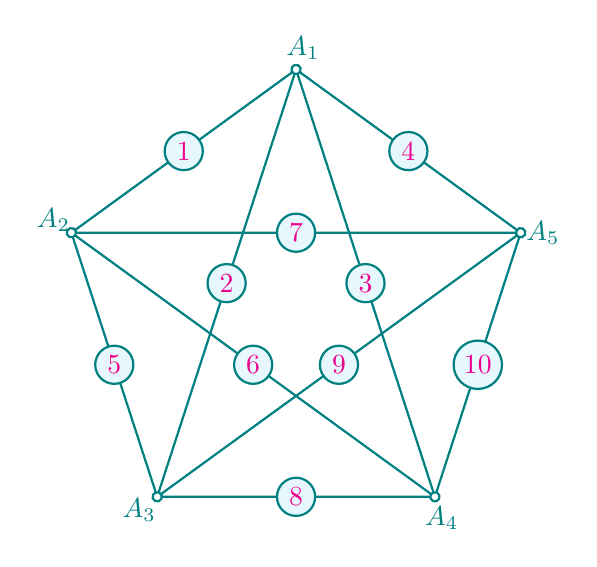
\begin{tikzpicture}[rotate=18,thick,teal]
		\def\n{5}
		\def\dd{3}
		\def\tong{0}
		\pgfmathsetmacro{\nt}{\n-1}
		\foreach \x in {1,2,...,\nt}{
			\pgfmathsetmacro{\xt}{\x+1}
			\foreach \y in {\xt,...,\n}{
				\pgfmathsetmacro{\so}{int(\tong+1)}
				\xdef\tong{\so}
				\draw (\x*360/\n:\dd)--(\y*360/\n:\dd) 
				node[draw,circle,inner sep =2pt,pos=0.5,fill=cyan!10]{\color{magenta}\tong};
			}
		}  
		\foreach \x in {1,2,...,\n}{
			\pgfmathsetmacro{\xt}{\x*360/\n}
			\draw[fill=white] (\xt:\dd) circle(1.69pt) node[shift={(\xt:8pt)}]{\color{teal}$A_\x$}; 
		}
	\end{tikzpicture}
	%%===========================================%%%
	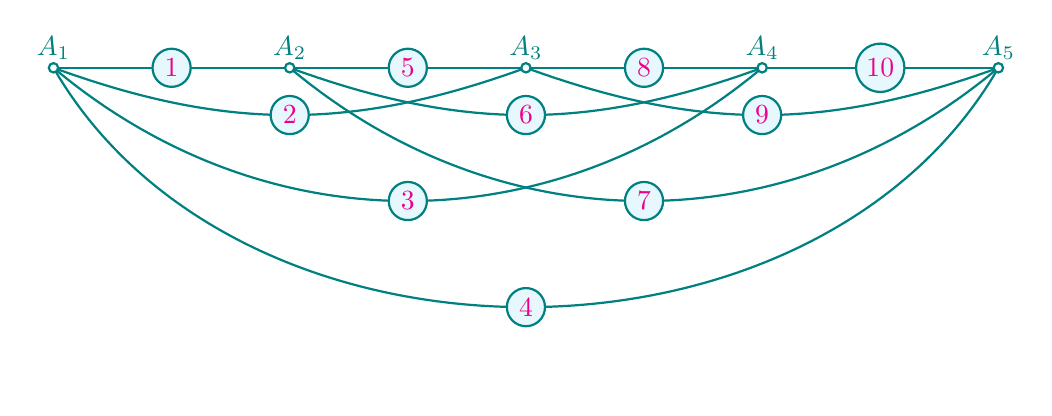
\begin{tikzpicture}[x=3cm,thick,teal]
		\def\n{5}
		\def\tong{0}
		\pgfmathsetmacro{\nt}{\n-1}
		\foreach \x in {1,2,...,\nt}{
			\pgfmathsetmacro{\xt}{\x+1}
			\foreach \y in {\xt,...,\n}{
				\pgfmathsetmacro{\di}{int(\y-\x-1)*(-20)}
				\pgfmathsetmacro{\vao}{180-\di}
				\pgfmathsetmacro{\so}{int(\tong+1)}
				\xdef\tong{\so}
				\draw (0:\x) to [out=\di,in=\vao] coordinate[pos=0.5] (At) (0:\y);
				\node[draw,circle,inner sep =2pt,fill=cyan!10] at (At) {\color{magenta}\tong};
		} }  
		\foreach \x in {1,2,...,\n}{
			\draw[fill=white] (0:\x) circle(1.69pt) node[shift={(90:7pt)}]{\color{teal}$A_\x$}; 
		}
	\end{tikzpicture}
\end{document}